\documentclass[tikz,border=5pt]{standalone}
\usepackage{amsmath}
\begin{document}
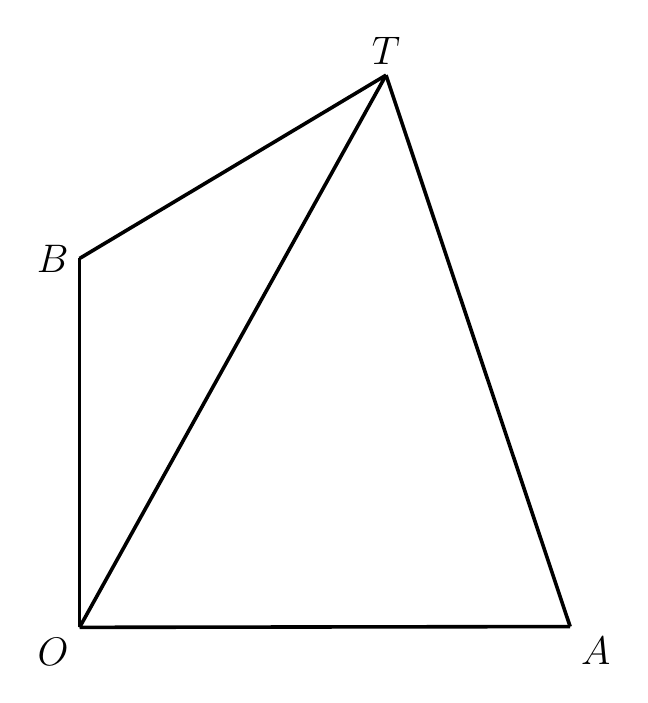
\begin{tikzpicture}[line join=round, line width=1.3pt]
  % Scale s = 0.016495 (from STYLE METRICS); origin at O
  \coordinate (O) at (0,0);
  \coordinate (A) at (6.230,0.010);
  \coordinate (T) at (3.892,7.013);
  \coordinate (B) at (0,4.685);

  % Triangle and vertical side
  \draw (O) -- (A);
  \draw (A) -- (T);
  \draw (T) -- (O);
  \draw (T) -- (B);
  \draw (O) -- (B);

  % Labels (14pt font per style metrics)
  \node[above, font=\fontsize{14}{16.8}\selectfont] at (T) {$T$};
  \node[left, font=\fontsize{14}{16.8}\selectfont] at (B) {$B$};
  \node[below left, font=\fontsize{14}{16.8}\selectfont] at (O) {$O$};
  \node[below right, font=\fontsize{14}{16.8}\selectfont] at (A) {$A$};
\end{tikzpicture}
\end{document}